\chapter{Experiments}

    \section{V1}

        \subsection{Spark ignition}
            
            As was discussed in \textcite{duplayArgonLaserPlasmaThruster2024a}, spark ignition was not reliable enough with the available electrode system. 

        \subsection{Bringing the pulsed power down and Optical design (move to design)} \label{sec:pulse_power_down_V1}
            
            Pulsed shots at lower power levels revealed a difficulty to ignite the LSP below \qty{20}{\%} power, which corresponds to about \qty{620}{W}. This poses a problem, as the maximum CW power of the laser is significantly lower, at \qty{350}{W}. A test campaign was started in February 2024 to determine if LSP ignition in the V1 thruster was possible under this maximum CW power level.
            
            To obtain LSP ignition, a high enough laser flux is needed. With a fixed power, it is necessary to focus the laser down to the smallest area possible to get the highest flux. Quantifying the diameter of this focus was therefore the first step. 

            %Section on quantifying diameter, laser optics basics (email from thorlabs guy)

            For a multi-element system, the spot diameter must be calculated numerically with ray tracing software. WinLens 3D Basic \cite{winlens} was used here, as it is free and powerful enough for this application. The single element system was also simulated in this software to verify the calculations.

            Now that the diameter of the focus is known, two avenues are possible to improve it: a shorter focal length or a multi-lens system \cite{thorlabs}. At first, a single lens with a \qty{125}{mm} focal length (Thorlabs LA1384-C \cite{125mm lens}) was used, as it was the simpler option. During these shots, the goal was to achieve LSP ignition at or below \qty{11}{\%} pulsed power, or \qty{340}{W}. The following graph shows LSP ignition attempts at various power settings and axial lens positions. 20 pulsed laser shots were performed for each point on the graph. If at least one was successful at igniting LSP, it was recorded as such. This graph can also be interpreted as a beam profiling for LSP conditions.
            
            % Graph of 125mm lens
            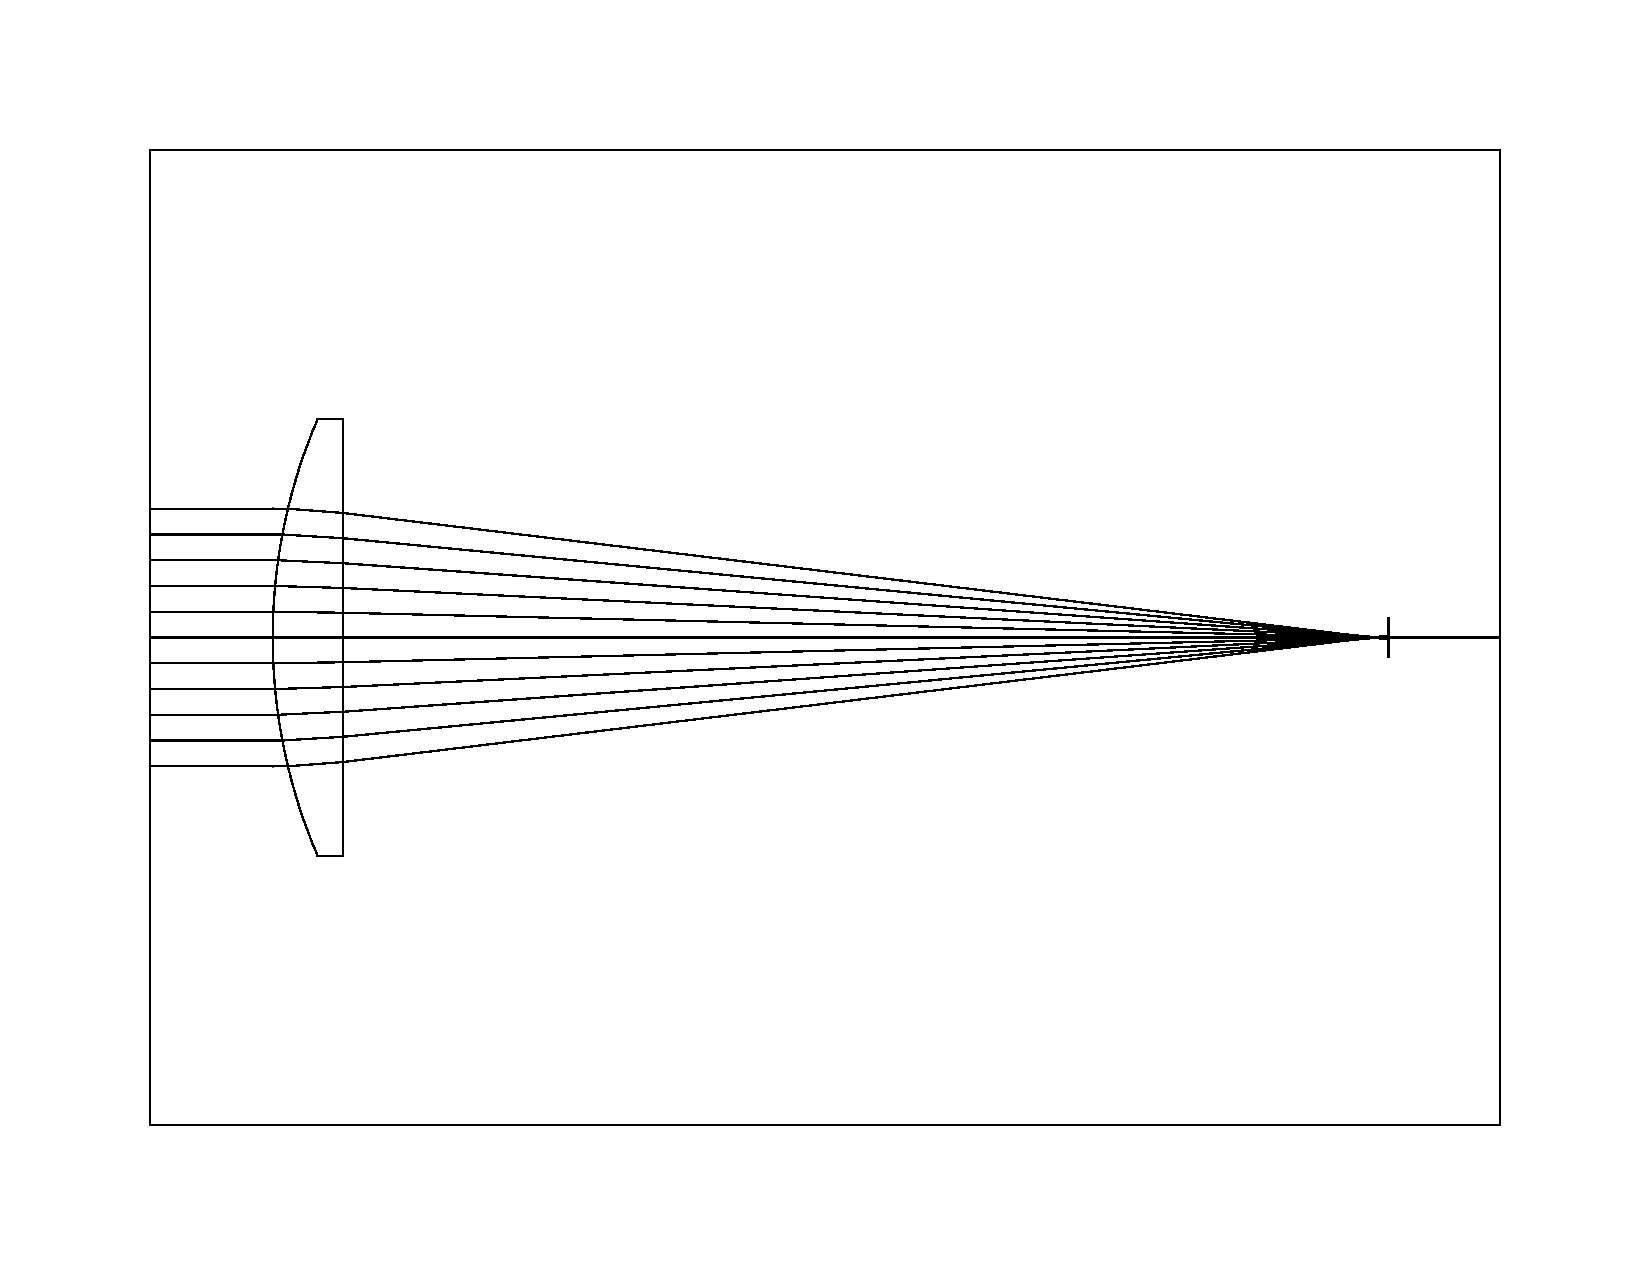
\includegraphics[width=\textwidth]{assets/5 results/125lens.pdf}

            \begin{figure}[h]
                \centering
                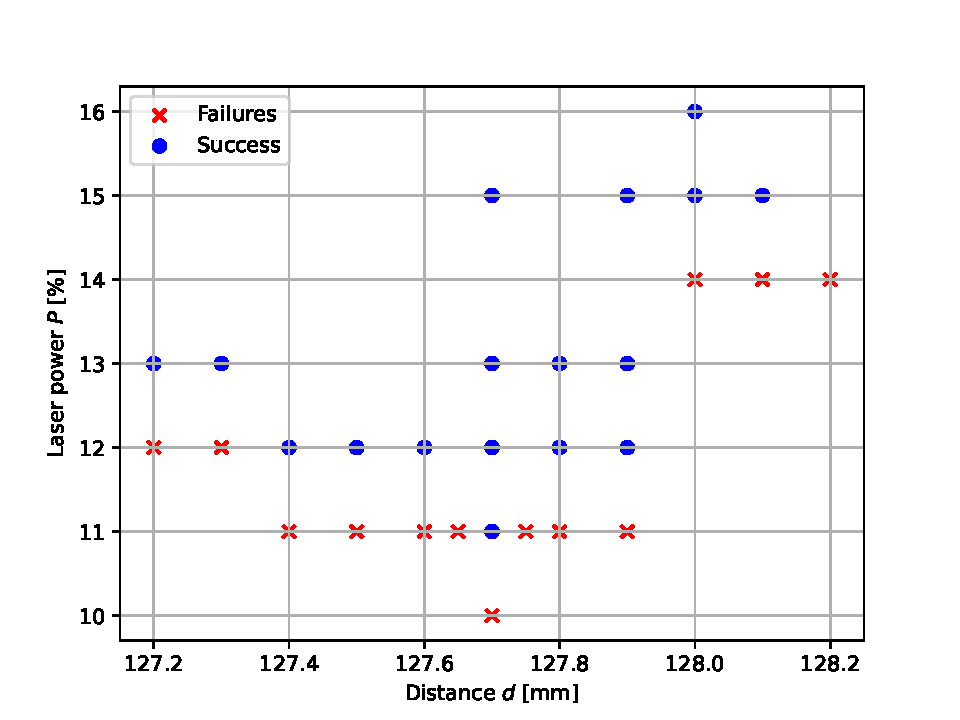
\includegraphics[width=0.75\textwidth]{assets/5 results/125mm_focus_threshold.pdf}
                \caption{125 mm focal length lens}
            \end{figure}
            
            Ignition at \qty{11}{\%} was attained once, but it was not possible to replicate this. A tighter focus was necessary to increase ignition reliability.

            % Graph of multi-lens
            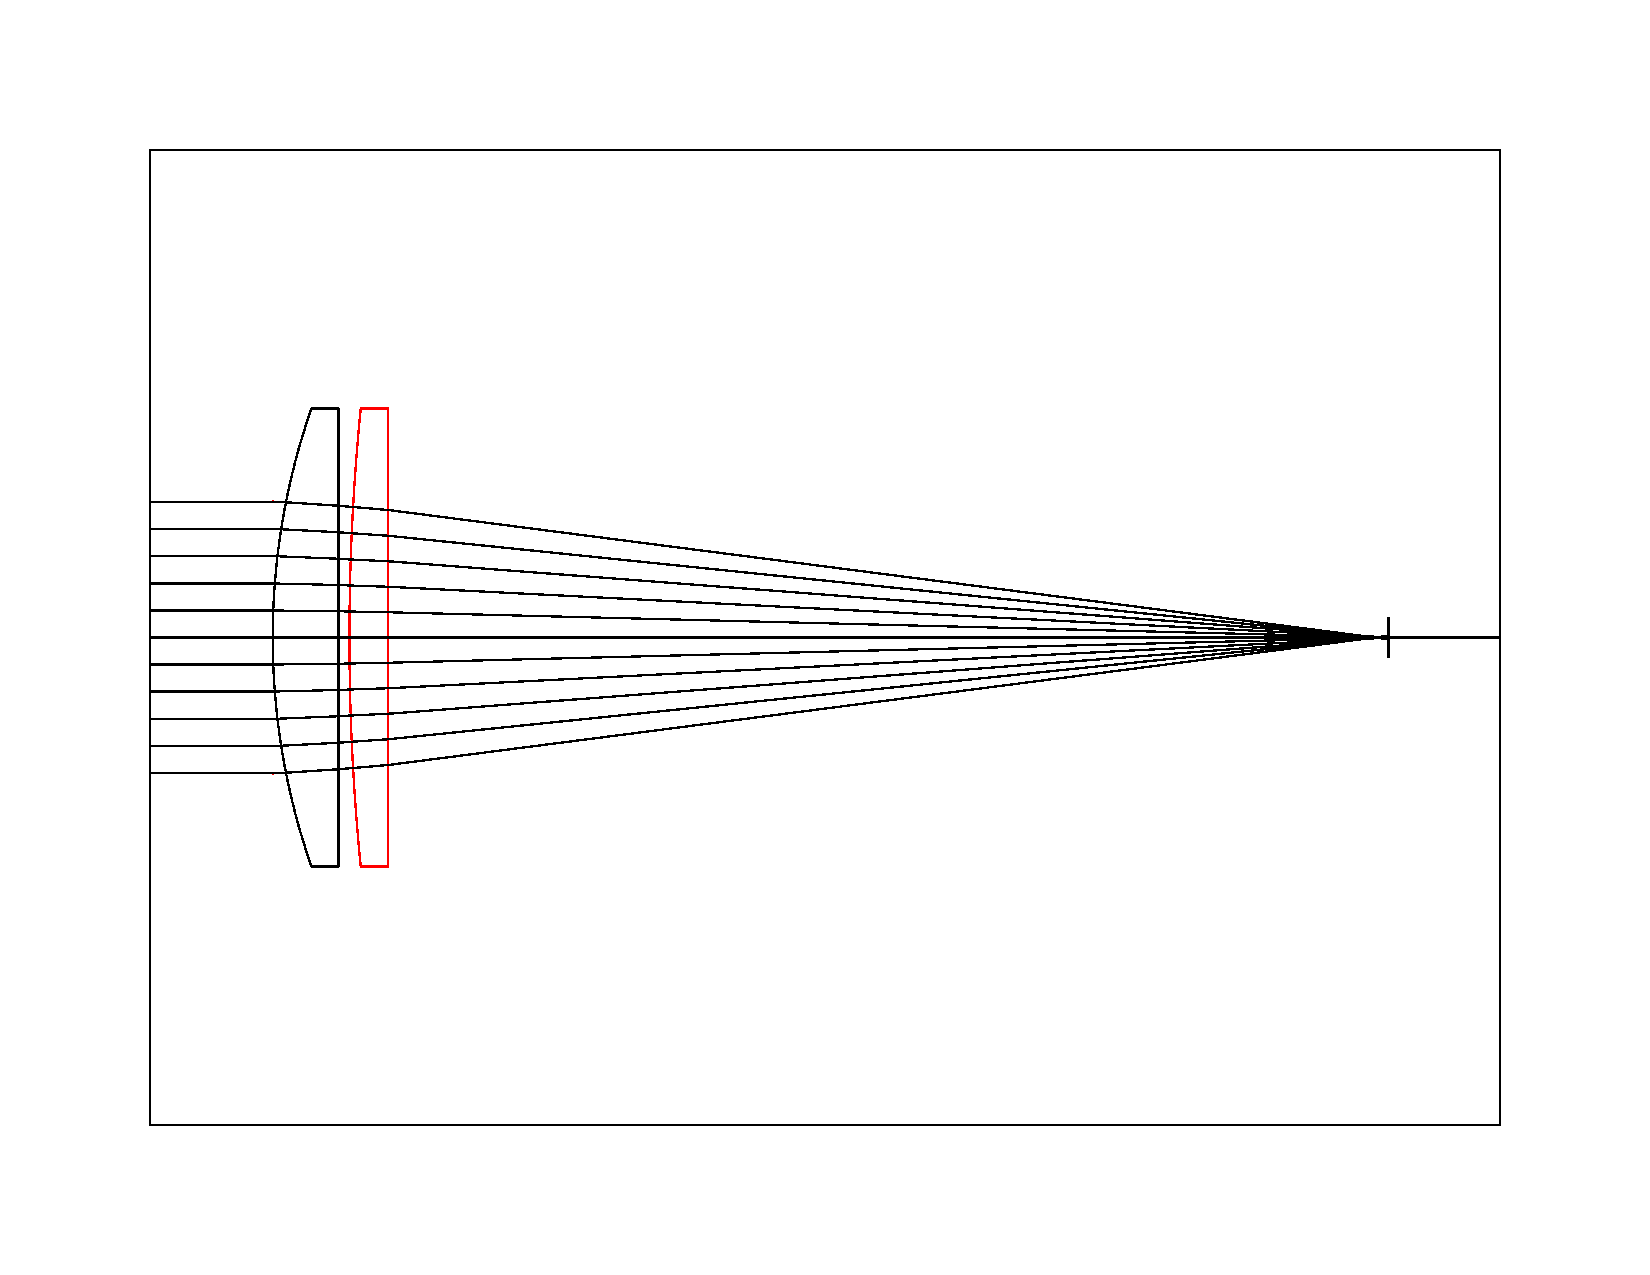
\includegraphics[width=\textwidth]{assets/5 results/500 and 150 lenses.pdf}

            \begin{figure}[h]
                \centering
                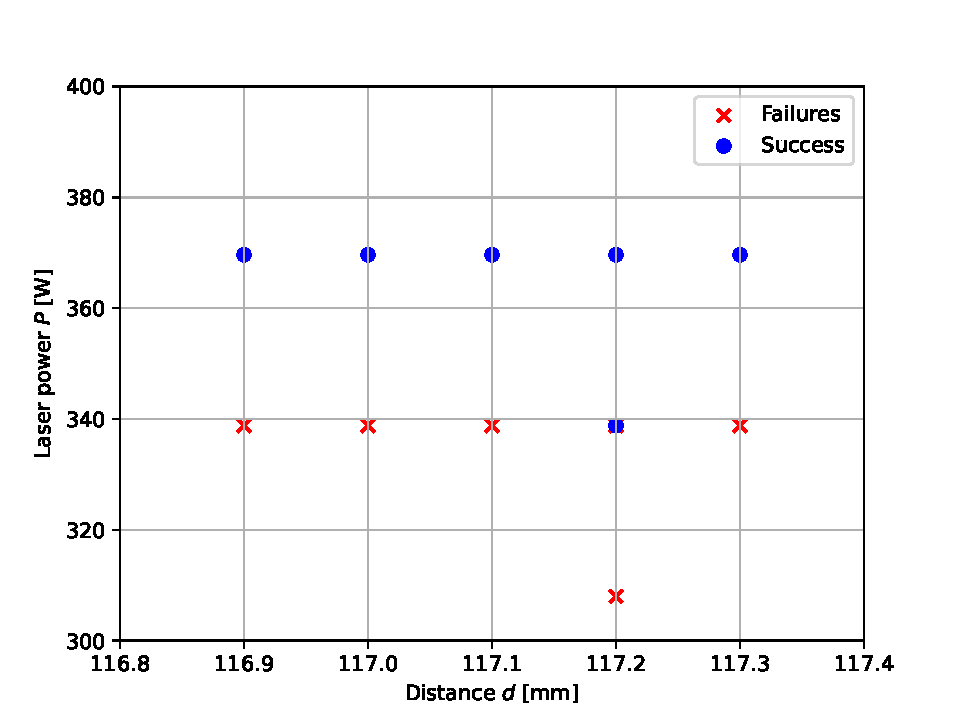
\includegraphics[width=0.75\textwidth]{assets/5 results/duallens_focus_threshold.pdf}
                \caption{Multi-lens system}
            \end{figure}

            % Section on power meter reading lower pulsed power at these low power settings, like about 200W

            The completion of these tests validated LSP generation in the CW power regime of the laser. The V2 thruster was then set up to ultimately test CW operation with flowing argon.
        
        \subsection{\ce{NO2} seeding}
            
            As the plasma emits in the ultraviolet (UV) range, it is necessary to seed with a gas that absorbs UV but not the infrared (IR) laser. \textcite{khanGasDetectionUsing2019} shows that \ce{NO2} and \ce{SO2} are two candidates. \ce{NO2} was first used as it was easy to produce in-house in significant quantities. The V1 system was set up with a vacuum pump connected to an outside air exhaust to safely vent the \ce{NO2} gas. The pump was also used to bring the pressure in the test section down to vacuum (how much?) before introducing gas.

            Control LSP shots were undertaken in pure argon. Next, 0.55 bar of \ce{NO2}, or 200 mL at STP, were introduced into the chamber. It was then pressurized with argon to 20 bar. With the spark active, LSPs were consistently generated in the seeded atmosphere and their pressure trace from the PCB transducer was recorded with the oscilloscope. This pressure rise was approximately double the one seen in pure argon; see \autoref{fig:NO2_shots_analysis}.

            The next series of LSP shots was conducted with 0.24 bar (\qty{85}{ml} at STP) of \ce{NO2} and filled to 20.2 bar of argon. Again, higher pressure rises were observed, but slightly less than the \qty{0.55}{bar} shots. The chamber was finally half evacuated to 10.17 bar and then filled back to \qty{20.15}{bar}. This should bring the partial pressure of \ce{NO2} to \qty{0.12}{bar}. Again, LSPs were consistent, with a higher pressure rise than pure argon, but less than the higher concentration \ce{NO2} shots.

            \begin{figure}[h]
                \centering
                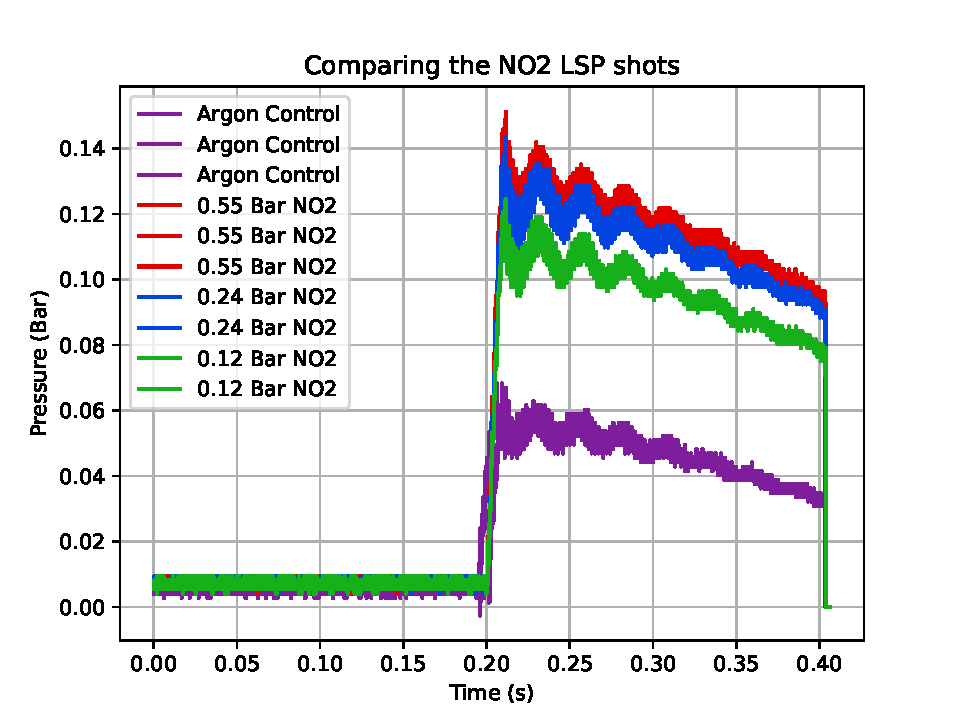
\includegraphics[width=0.75\textwidth]{assets/5 results/NO2_shots_analysis.pdf}
                \caption{NO2 LSP shots}
                \label{fig:NO2_shots_analysis}
            \end{figure}

            Indeed, with as low as (0.5\%?) of \ce{NO2} mixed with argon, nearly double the pressure rise is observed. This indicates that the working gas is absorbing twice the energy from the plasma. As the \ce{NO2} fraction is increased, there are diminishing returns to the pressure rise. This is encouraging, as not much \ce{NO2} is needed to have a great impact on the energy absorption.

    \section{V2}
        This section presents the various experiments that were conducted with the V2 thruster.
    
        \subsection{Initial LSP shots}

            \begin{figure}
                \centering
                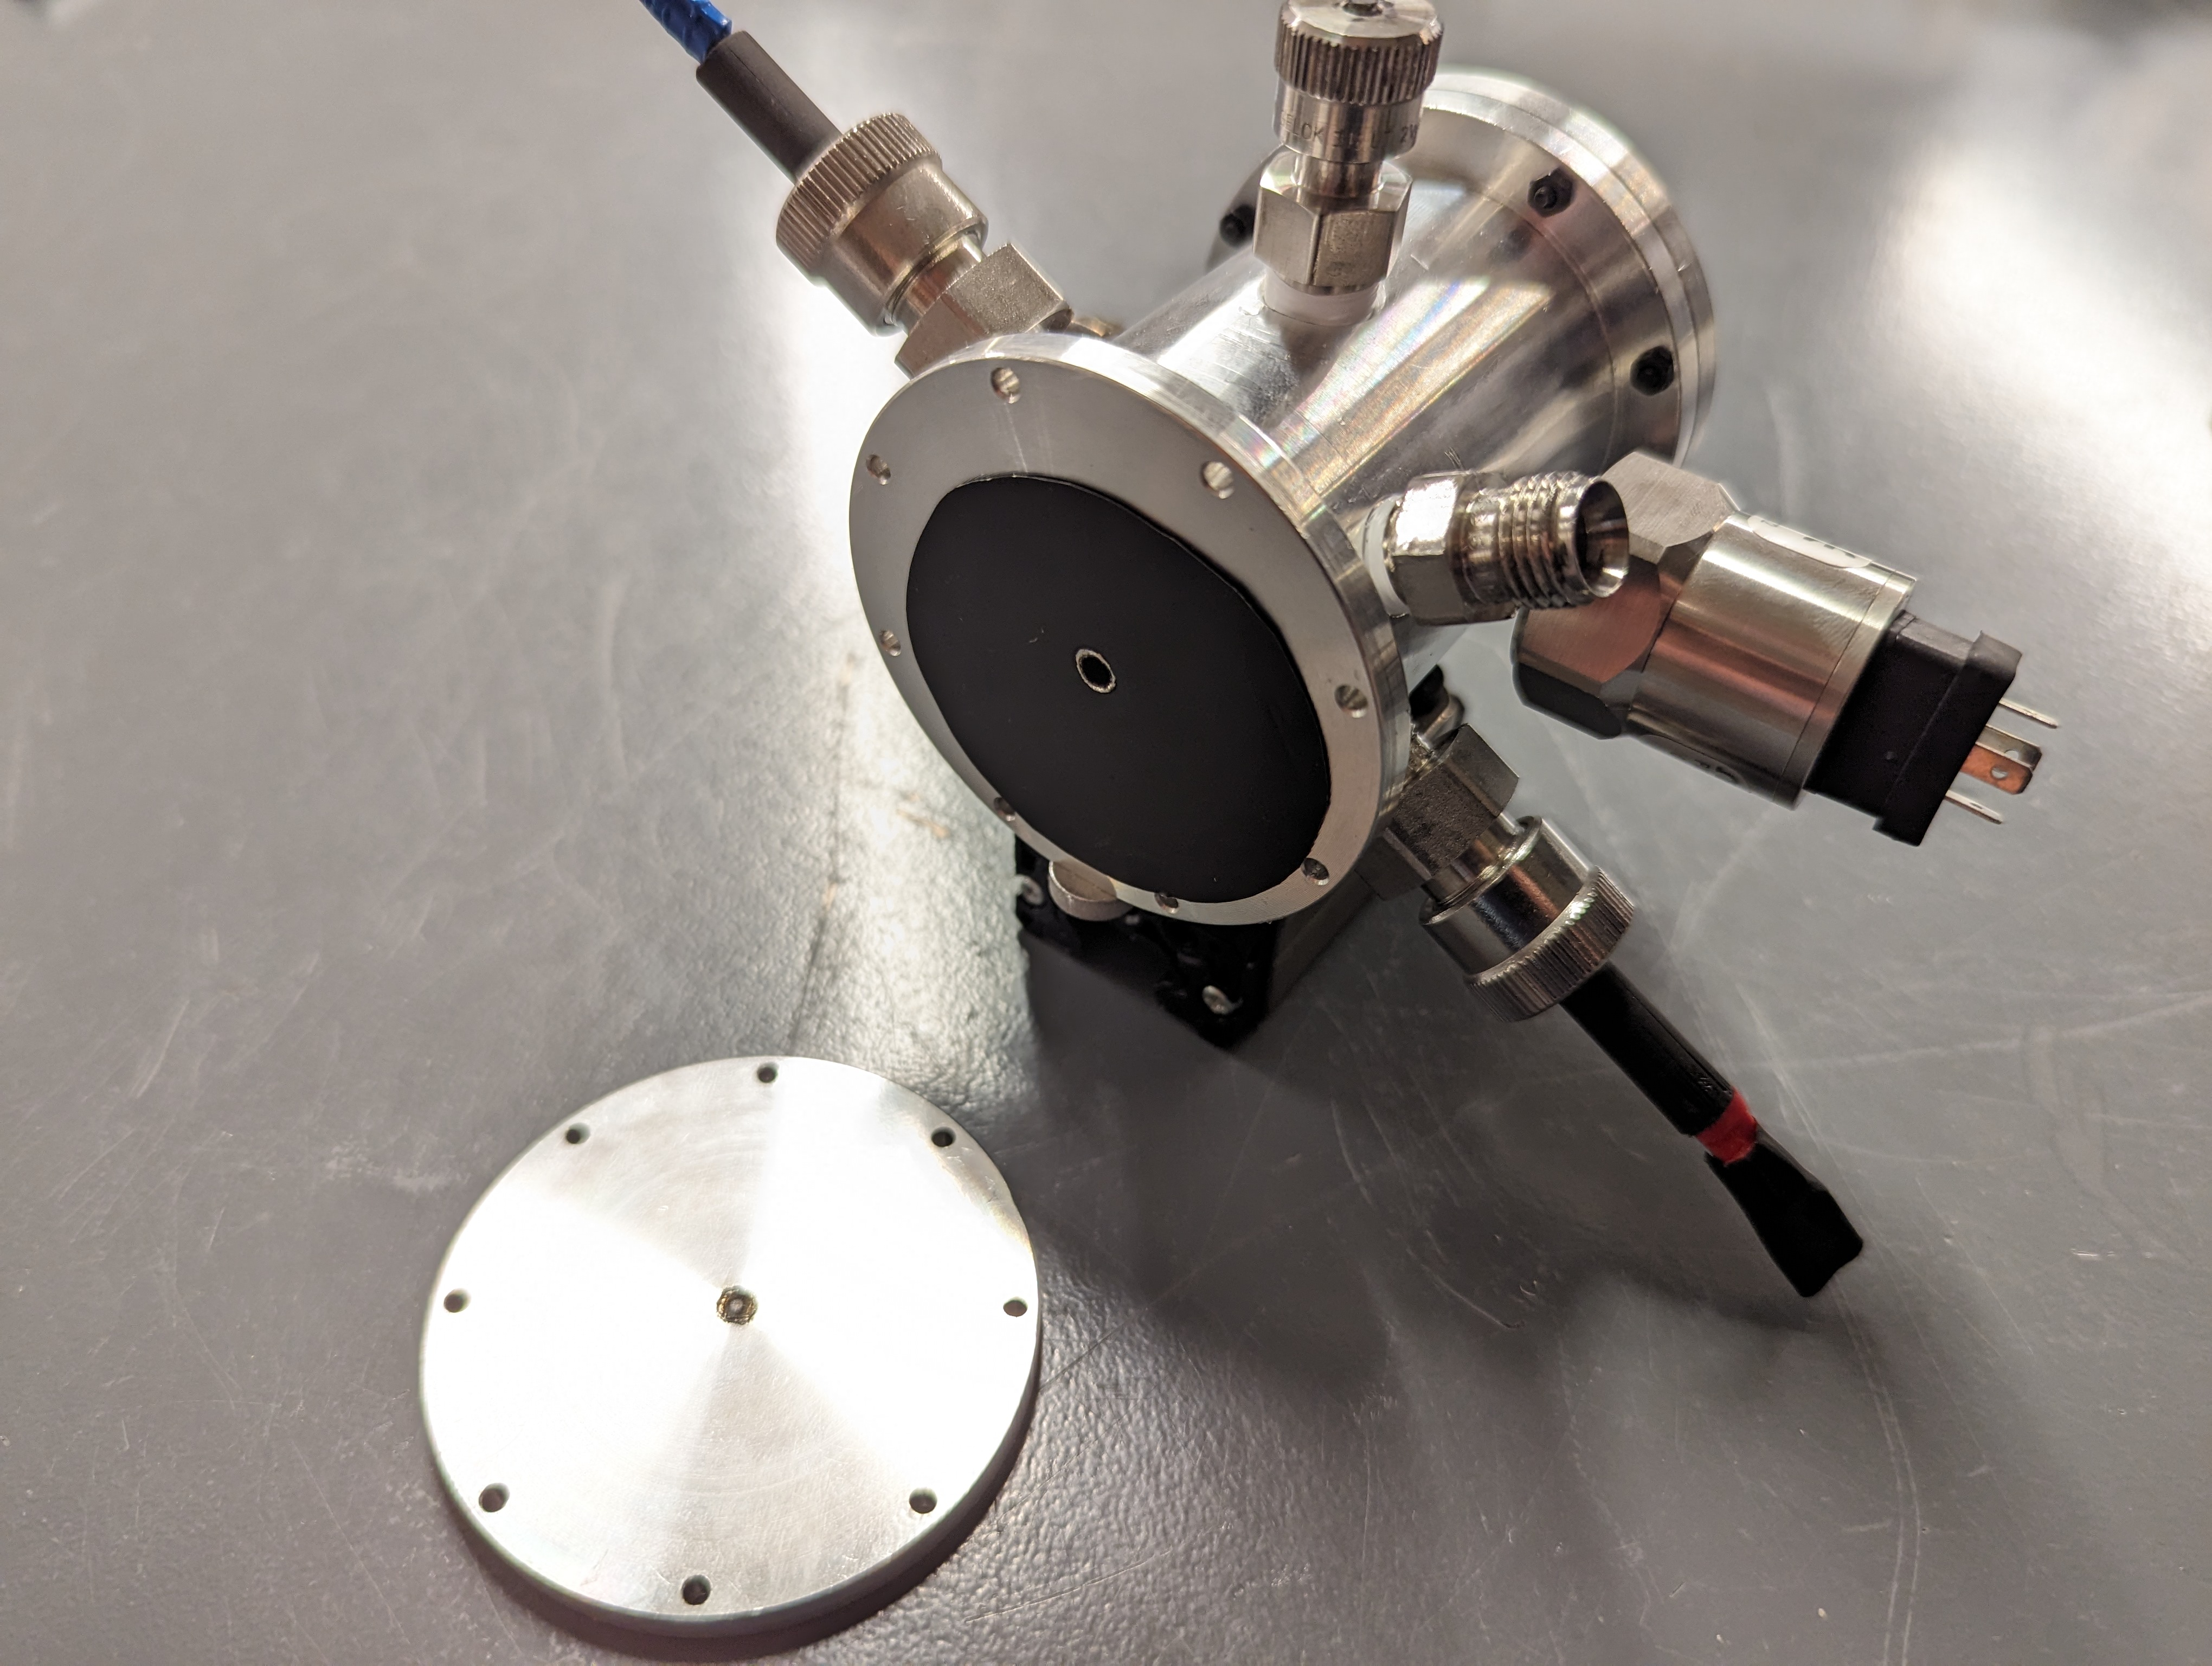
\includegraphics[width=0.75\textwidth]{assets/5 results/V2 test damage.jpg}
                \caption{Damage to the thruster after two \qty{3}{kW} laser shots}
            \end{figure}

            % Stills of first High-speed LSP video, showing expansion of LSP wave like in V1
        
        \subsection{Cold flow thrust tests}

            Cold flow tests were completed to give a baseline measurement of thrust before the hot fire test, and to validate the functioning of all data acquisition systems.
            
            % thrust vs pressure graph

        \subsection{Bringing the pulsed power down, again}
            
            To prevent the damage to the thruster seen previously, a rear window mount was manufactured. This allows the laser energy that is not absorbed to pass freely through the apparatus, also enabling power meter measurements. The following figures present the LSP ignition attempts with focus distance, similarly to the graphs presented in \autoref{sec:pulse_power_down_V1}. 
 

            

        



